\usetikzlibrary{shapes.geometric, arrows, shapes.misc}

\tikzstyle{input} = [rectangle, rounded corners, minimum width=3cm, minimum height=1cm,text centered, draw=black, fill=blue!10,  align=center]
\tikzstyle{software} = [
        chamfered rectangle,
        chamfered rectangle xsep=2cm,
        minimum width=3cm, minimum height=1cm, text centered, draw=black, fill=orange!30]
\tikzstyle{interm} = [rectangle, rounded corners, minimum width=3cm, minimum height=1cm,text centered, draw=black, fill=red!10,  align=center] 

\tikzstyle{output} = [circle, minimum width=3cm, minimum height=1cm, text centered, draw=black, align=center, fill=green!10]
\tikzstyle{arrow} = [thick,->,>=stealth]

\begin{figure}
\centered
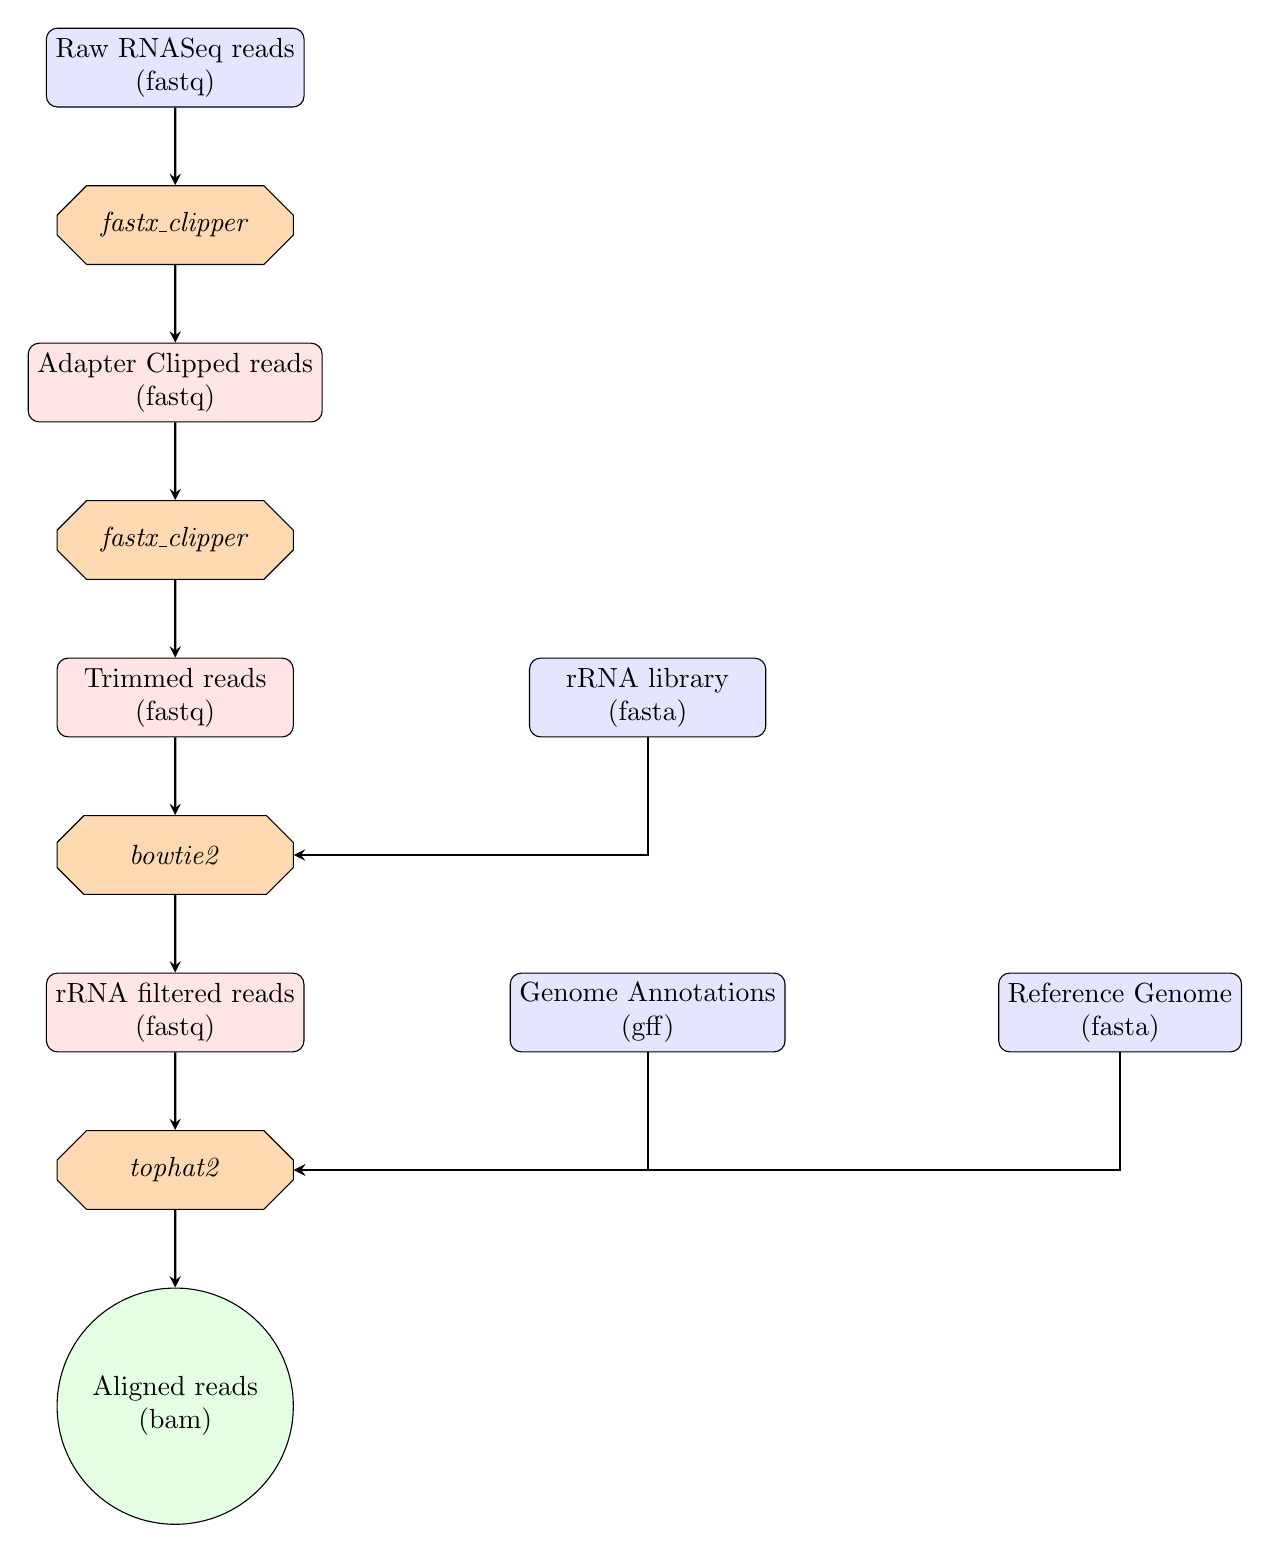
\begin{tikzpicture}
\node (fasta_raw) [input] {Raw RNASeq reads \\ (fastq)};
\node (clipper) [software, below of=fasta_raw, yshift=-1cm] {\textit{fastx\_clipper}};

\node (clipped) [interm, below of=clipper, yshift=-1cm] {Adapter Clipped reads\\ (fastq)};

\node (trimmer) [software, below of=clipped, yshift=-1cm] {\textit{fastx\_clipper}};

\node (trimmed) [interm, below of=trimmer, yshift=-1cm] {Trimmed reads\\ (fastq)};

\node (rrna) [input, right of=trimmed, xshift=5cm] {rRNA library \\ (fasta)};

\node (rrna_filter) [software, below of=trimmed, yshift=-1cm] {\textit{bowtie2}};

\node (filtered) [interm, below of=rrna_filter, yshift=-1cm] {rRNA filtered reads\\ (fastq)};

\node (genome_gff) [input, right of=filtered, xshift=5cm] {Genome Annotations \\ (gff)};
\node (genome_fa) [input, right of=genome_gff, xshift=5cm] {Reference Genome \\ (fasta)};


\node (tophat) [software, below of=filtered, yshift=-1cm] {\textit{tophat2}};

\node (bam) [output, below of=tophat, yshift=-2cm] {Aligned reads \\ (bam)};


\draw [arrow] (fasta_raw) -- (clipper);
\draw [arrow] (clipper) -- (clipped);

\draw [arrow] (clipped) -- (trimmer);
\draw [arrow] (trimmer) -- (trimmed);

\draw [arrow] (trimmed) -- (rrna_filter);
\draw [arrow] (rrna) |- (rrna_filter);
\draw [arrow] (rrna_filter) -- (filtered);

\draw [arrow] (filtered) -- (tophat);
\draw [arrow] (genome_gff) |- (tophat);
\draw [arrow] (genome_fa) |- (tophat);
\draw [arrow] (tophat) -- (bam);

\end{tikzpicture}
\caption{M1} \label{fig:M1}
\end{figure}
